../cictikz/src/cictikz/data/tex/cictikz_preamble.tex

% Temperature behaviour of AT cut crystals: the classic family of
% S-curves, antisymmetric about the ~25 C inflection point. The linear
% term is set by the cut angle error, the cubic term by the crystal, so
% the closer the cut is to the flat curve, the more expensive the part.
% Model: df/f [ppm] = 1.05e-4*(T-25)^3 - s*(T-25).

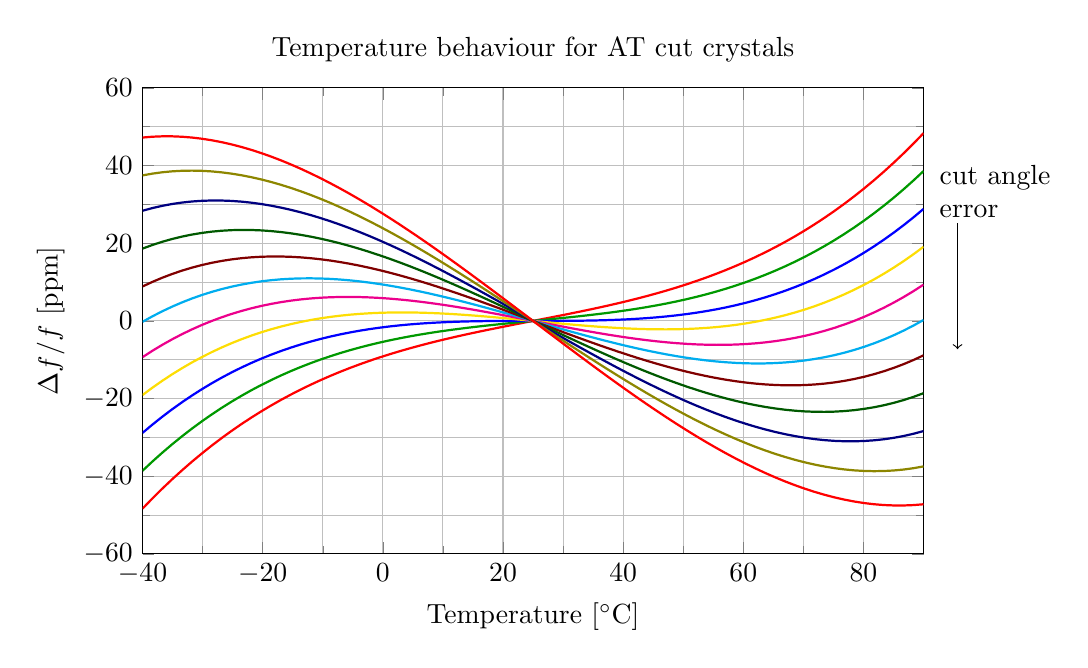
\begin{tikzpicture}
  \begin{axis}[
    width=11.5cm, height=7.5cm,
    xlabel={Temperature [$^\circ$C]},
    ylabel={$\Delta f/f$ [ppm]},
    title={Temperature behaviour for AT cut crystals},
    xmin=-40, xmax=90, ymin=-60, ymax=60,
    grid=both,
    minor tick num=1,
    domain=-40:90, samples=80,
    every axis plot/.append style={thick, no marks},
    cycle list={red,green!60!black,blue,yellow!80!orange,magenta,cyan,
                red!50!black,green!35!black,blue!50!black,olive},
  ]
    \foreach \s in {-0.30,-0.15,0.0,0.15,0.30,0.44,0.58,0.73,0.88,1.02,1.17} {
      \addplot+ {1.05e-4*(x-25)^3 - \s*(x-25)};
    }
  \end{axis}

  % what separates the curves
  \node[anchor=west, align=left] at (10.0,4.6)
    {cut angle\\error};
  \draw[->] (10.35,4.2) -- (10.35,2.6);

\end{tikzpicture}
\end{document}
